%%%%%     PACKS     %%%%%
\documentclass[12pt]{article}
\usepackage[margin=1in,headsep=.60in]{geometry}
\usepackage[utf8]{inputenc}
\usepackage[table, dvipsnames]{xcolor}
\usepackage{array}
\usepackage{amsmath}
\usepackage{booktabs}
\usepackage{mdframed} %For box around text
\usepackage{hyperref} %For hyperlinks in the PDF
\hypersetup{
    colorlinks=true,
    linkcolor=blue,
    filecolor=magenta,
    urlcolor=cyan,
}
\urlstyle{same}
\usepackage{amsthm}
\usepackage{amssymb}
\usepackage{amsfonts}
\usepackage{siunitx}
\usepackage{graphicx}
\usepackage{caption}
\usepackage{pgfplots}
\graphicspath{{Images/}}
\usepackage[colorinlistoftodos]{todonotes}
\usepackage{cleveref}
\usepackage[labelformat=simple]{subcaption}
\usepackage{grffile}
\usepackage{gensymb}
\usepackage{float}
\usepackage[shortlabels]{enumitem}
\usepackage{enumitem}
\setlistdepth{9}
\usepackage{biblatex} %Imports biblatex package
\addbibresource{references.bib}
\usepackage{outlines}
\usepackage{minted}
\usepackage{pdflscape}
\usepackage{everypage}
\usepackage{multirow}
\usepackage{multicol}
\usepackage{afterpage}
\usepackage[labelfont=bf, font=small]{caption}
\usepackage{upgreek}
\usepackage{tikz}
\usepackage{xcolor}
\usepackage{listings}

% style sheet for code
\definecolor{codegreen}{rgb}{0,0.6,0}
\definecolor{codegray}{rgb}{0.5,0.5,0.5}
\definecolor{codepurple}{rgb}{0.58,0,0.82}
\definecolor{backcolour}{rgb}{0.95,0.95,0.92}

\lstdefinestyle{mystyle}{
    backgroundcolor=\color{backcolour},   
    commentstyle=\color{codegreen},
    keywordstyle=\color{magenta},
    numberstyle=\tiny\color{codegray},
    stringstyle=\color{codepurple},
    basicstyle=\ttfamily\footnotesize,
    breakatwhitespace=false,         
    breaklines=true,                 
    captionpos=b,                    
    keepspaces=true,                 
    numbers=left,                    
    numbersep=5pt,                  
    showspaces=false,                
    showstringspaces=false,
    showtabs=false,                  
    tabsize=2
}

\lstset{style=mystyle}

\usepackage{lastpage}
%%%%%     COMMANDS     %%%%%
%%%% Blue box for subsection text (not figures) %%%%
\newenvironment{bluebox}
  {\begin{mdframed}[backgroundcolor=blue!5,linecolor=blue!40,roundcorner=8pt]}
  {\end{mdframed}}

%%%% Simple neutral box for figures %%%%
\newenvironment{figbox}
  {\begin{mdframed}[roundcorner=8pt,shadow=true,shadowsize=4pt,shadowcolor=black!40]}
  {\end{mdframed}}

\begin{document}

\begin{titlepage}
\newcommand{\HRule}{\rule{\linewidth}{0.5mm}}

\center

\textsc{\LARGE Aarhus University}\\[1.5cm]
\textsc{\Large Computer Science}\\[0.5cm]
\textsc{\large Numerical Linear Algebra}\\[0.5cm]
    

\HRule\\[0.4cm]
    \center 
    {\huge\bfseries Handin 9 }\\[0.4cm] % Title of your document
\HRule\\[1.5cm]

\begin{minipage}{0.4\textwidth}
        \begin{flushleft}
            \large
            \textit{Author}\\   
            Søren M. \textsc{Damsgaard}\\
                 % Your name
        \end{flushleft}
    \end{minipage}
~
    \begin{minipage}{0.4\textwidth}
        \begin{flushright}
            \large
            \textit{Student number}\\
            \textbf{202309814}\\
                 % Studienummer\
            
        \end{flushright}
    \end{minipage}

\vfill\vfill\vfill % Position the date 3/4 down the remaining page
    
    {\large\today}

\vfill\vfill
    
\includegraphics[width=0.2\textwidth]{Aarhus_University_seal.png}\\[1cm] % Include a department/university logo - this will require the graphicx package
    

\vfill
\end{titlepage}
%%%%%      CHAPTERS      %%%%%
\hspace{0.02cm}
\section*{Zulu Bravo PsyOp Striker 9}
Given a system of flowing thingies~\ref{fig:flow} with the following information:
\begin{enumerate}
    \item $A$ contains $300\; L$ of mixture and $84 \; g$ of salt.
    \item $B$ contains $100 \; L$ of muxture and $36 \; g$ of salt.
    \item $a$ flows with $30\; L\slash\min$ of water
    \item $b$ flows with $15 \; L \slash\min$ of mixture
\end{enumerate}
\begin{figure}[H]
    \centering
    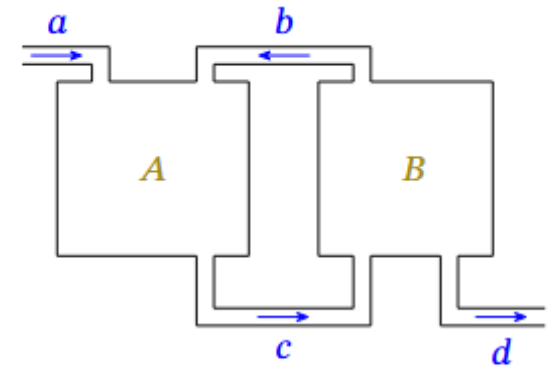
\includegraphics[width=0.8\textwidth]{flowchart.png}
    \caption{Containers connected  by pipes: Flowchart of the system.}
    \label{fig:flow}
\end{figure}
\subsection*{The Equalizer}
Determining the flow of $c$ and $d$ so as the amount of liquid in both containers are constant.
\begin{enumerate}
    \item \textbf{$A$} has an input $a$ and $b$ which totals to $45 \; L \slash\min$, so $c$ needs to flow with $45 \; L \slash\min$ to cancel out the input from $a$ and $b$.
    \item \textbf{$B$} has an output $b$ and a newly determined input $c$, so the following should determine the flow of the remaining pipe $c-b = 30 \; L \slash\min = d$ 
\end{enumerate}
\subsection*{Two Peens In A System}
Explain why the salt amounts $y_0(t)$ in $A$ and $y_1(t)$ in $B$ satisfy the system
\begin{align*}
    y'_0(t) &= -0.15y_0(t) + 0.15y_1(t)\\
    y'_1(t) &= 0.15y_0(t) - 0.45y_1(t)
\end{align*}
The change in salt corresponds to the input and output, percentages, of mixture in each container.\\
for $A$: $c$ outputs $45 \; L \slash\min$ which is $15\%$ of $A$ hence $-0.15y_0(t)$, and $b$ inputs $15 \; L \slash\min$ which is $15\%$ of $B$ hence $+0.15y_1(t)$.\\
for $B$: $c$ inputs so it's $+0.15y_0(t)$ and $b$ outputs $45 \; L \slash\min$ which is $45\%$ of $B$ hence $-0.45y_1(t)$.\\\\
This give us a system that can be written as:
\begin{equation*}
    y'(t)=Ay = \begin{bmatrix}-0.15 & 0.15\\
0.15 & -0.45\end{bmatrix} \begin{bmatrix}y_0(t)\\
y_1(t)\end{bmatrix}
\end{equation*}
with the initial value:
\begin{equation*}
    y(0) = \begin{bmatrix}
        84 \\
        36 
    \end{bmatrix}
\end{equation*}

\subsection*{To Eigen or Not To Eigen}
The Author calls upon god to protect me against the horros and impending doom of using a numpy function that isn't explicitely shown in the Bibel of Numerical Linear Algebra by Jesus AKA Andrew Swan.\\\\
\begin{lstlisting}[language=Python]
import numpy as np

A = np.array([[-0.15, 0.15], 
              [0.15, -0.45]])
# Please don't end me... \(;_;)/
eigvalues, eigvectors = np.linalg.eig(A)

print('Eig Values:\n', eigvalues)
print('Eig Vectors:\n', eigvectors)

# Output (not part of the actual code, just for reference):
Eig Values:
 [-0.08786797 -0.51213203]
Eig Vectors:
 [[ 0.92387953 -0.38268343]
 [ 0.38268343  0.92387953]]
\end{lstlisting}
Reducing the Eig thingies to just two significant values.
\begin{equation}\label{EigVal}
   \text{Eigenvalues} \qquad \lambda_0 = -0.09 \qquad \lambda_1 = -0.51
\end{equation}
\begin{equation}\label{EigVec}
    \text{Eigenvectors} \qquad
    v_0 =
    \begin{bmatrix}
        0.92 \\
        0.38
    \end{bmatrix}
    \qquad 
    v_1 =
    \begin{bmatrix}
        -0.38 \\
        0.92
    \end{bmatrix}
\end{equation}

\subsection*{Solutions for $y_0(t)$ and $y_1(t)$}
Finding a solution for $y'_0(t)$ and $y'_1(t)$ using the eigen thingies, proposition 22.3~\cite{NUMLA} says a solution is given using the eigenvalues and eigenvectors as such:
\begin{equation*}
    y(t) = c_0v_0e^{\lambda_0 t} + c_1v_1e^{\lambda_1 t}
\end{equation*}
Inserting the values from \eqref{EigVal} and \eqref{EigVec}.
\begin{equation} \label{solution}
    y(t) = c_0  \begin{bmatrix}
        0.92 \\
        0.38
    \end{bmatrix} e^{-0.09t} + c_1 \begin{bmatrix}
        -0.38 \\
        0.92
    \end{bmatrix} e^{-0.51t}
\end{equation}
To isolate and determine $c_0$ and $c_1$, the initial state for $y(0)$ can be used.
\begin{equation*}
    y(0) = \begin{bmatrix}
        84 \\
        36
    \end{bmatrix} = c_0  \begin{bmatrix}
        0.92 \\
        0.38
    \end{bmatrix} + c_1 \begin{bmatrix}
        -0.38 \\
        0.92
    \end{bmatrix} = \begin{bmatrix}
        c_0 \cdot 0.92 + c_1 \cdot -0.38 \\
        c_0 \cdot 0.38 + c_1 \cdot -0.92
    \end{bmatrix}
\end{equation*}
This gives us the following system:
\begin{align*}
    0.92c_0 - 0.38c_1 &= 84 \\
    0.38c_0 + 0.92c_1 &= 36
\end{align*}
Using the god-given gift of numpy:
\begin{lstlisting}[language=Python]
B = np.array([[0.92, -0.38], 
              [0.38, 0.92]])

b = np.array([84, 36])

c0, c1 = np.linalg.solve(A, b)

print('c0 = ', c0)
print('c1 = ', c1)

# Output for reference (not part of the actual code)
c0 = 91.80460234154218
c1 = 1.2111425111021366
\end{lstlisting}
Rounding down $c_0$ and $c_1$
\begin{equation*}
    c_0 = 91.80 \qquad c_1 = 1.21
\end{equation*}
Now it's possible to determine a solution for both $y_0(t)$ and $y_1(t)$, by using the newfound constants and plotting them into \eqref{solution}
\begin{equation*}
   y(t) =
    91.80  \begin{bmatrix}
        0.92 \\
        0.38
    \end{bmatrix} e^{-0.09t} + 1.21 \begin{bmatrix}
        -0.38 \\
        0.92
    \end{bmatrix} e^{-0.51t} = \begin{bmatrix}
84.456e^{-0.09t} - 0.4598e^{-0.51t} \\
34.884e^{-0.09t} + 1.1132e^{-0.51t}
\end{bmatrix}
\end{equation*}
\subsection*{Plotting}
Plotting both $y_0$ and $y_1$ versus time, shows an exponential decrease in salt over time which is expected since the biggest term $-0.45$ represents the output in container B from pipe $d$.
\begin{figure}[H]
    \centering
    
\includegraphics[width=0.8\textwidth]{Figure_1.png}
    \caption{}
    \label{fig:time}
\end{figure}
For the $y_0$ versus $y_1$ it shows the relation in how the containers salt levels are related.
\begin{figure}[H]
    \centering
    
\includegraphics[width=0.8\textwidth]{Figure_2.png}
    \caption{}
    \label{fig:comp}
\end{figure}
This specifically shows a linear relation in the salt levels, since both container $A$ and $B$ drain the same rate over time.
\subsection*{Limits of $\infty$}
Taking \eqref{solution} and splitting it into $y_0$ and $y_1$
\begin{align*}
    y_0(t) &=c_0 0.92 e^{-0.09t} - c_1 0.38  e^{-0.51t} \\
    y_1(t) &=c_0 0.38 e^{-0.09t} + c_1 0.92 e^{-0.51t}
\end{align*}
it's know that $e^{-t} \to 0$ as $t \to \infty$ so the solution will approach zero as $t$ grows, which makes sense in regards to \ref{fig:time} and \ref{fig:comp}.\\
It also means that the terms that decay the fastest can be seen as neglible, so any terms with $e^{-0.51t}$
\begin{equation} \label{inf}
   \lim_{t \to \infty} \frac{y_1(t)}{y_0(t)} = \frac{c_0 0.38e^{-0.09t}}{c_0 0.92e^{-0.09t}} = \frac{0.38}{0.92} \approx 0.41
\end{equation}
Which is the ratio between the salt level in $A$ and $B$ as $t$ changes.




\section*{Appendix}
\begin{lstlisting}[language=Python]
import numpy as np
import matplotlib.pyplot as plt

# Finding Eigenvalues/vectors (c)
A = np.array([[-0.15, 0.15], 
              [0.15, -0.45]])
# Please don't end me... \(;_;)/
eigvalues, eigvectors = np.linalg.eig(A)


# solving for the constants c_0 and c_1 in (d)
B = np.array([[0.92, -0.38], 
              [0.38, 0.92]])

    b = np.array([84, 36])

c0, c1 = np.linalg.solve(B, b)


# (e)
t = np.linspace(0,100,1000)
y_0 = 84.456 * np.e**(-0.09*t) - 0.4598 * np.e**(-0.51*t)
y_1 = 34.884 * np.e**(-0.09*t) + 1.1132 * np.e**(-0.51*t)


## Brr brrr printing section
print(f'Eig Values:\n {eigvalues}')
print(f'Eig Vectors:\n {eigvectors}' )
print('c0 = ', c0)
print('c1 = ', c1)

fig1, y = plt.subplots()
y.plot(t,y_0, color='pink', label='Container A')
y.plot(t, y_1, color='purple', label='Container B')
y.set_title('Amount of salt in containers over time')
y.set_xlabel('Time')
y.set_ylabel('Salt Amount(g)')
y.grid()
y.legend()

fig2, pl = plt.subplots()
pl.plot(y_0,y_1, color='peru')
pl.set_xlabel('Salt amount in container A')
pl.set_ylabel('Salt amount in container B')
pl.grid()
pl.set_title('Salt amount in both containers in relation to each other over time')

plt.show()    
\end{lstlisting}
\printbibliography
\end{document}